\documentclass[11pt]{pnas-new}
% \documentclass[10pt]{article}
\templatetype{pnasresearcharticle} % Choose template 
% {pnasresearcharticle} = Template for a two-column research article
% {pnasmathematics} %= Template for a one-column mathematics article
% {pnasinvited} %= Template for a PNAS invited submission

\usepackage[utf8]{inputenc}
\usepackage[T1]{fontenc}
\usepackage{xcolor,ulem}
\usepackage{mdframed}
\usepackage{wrapfig}
\usepackage{multicol}
\setlength{\columnsep}{1cm}
\usepackage{graphicx}

\author[1]{Yoav Freund}
\author[2]{Hau-Tieng Wu}
\affil[1]{UCSD, department, city, postcode, country}
\affil[2]{Duke, department, city, postcode, country}

\title{Sometimes the digital Doctor should admit\\ "I don't know"}

\newcommand{\comment}[3]{{\color{#1} {\bf #2 :} #3}}
%\newcommand{\comment}[3]{}  % suppress comments
\newcommand{\hautieng}[1]{\comment{blue}{Hautieng}{#1}}
\newcommand{\yoav}[1]{\comment{red}{Yoav}{#1}}

\mdfsetup{middlelinecolor=blue, middlelinewidth=2pt, backgroundcolor=blue!10, roundcorner=10pt}

\mdfdefinestyle{Medicine}{middlelinecolor=red, middlelinewidth=2pt, backgroundcolor=red!10, roundcorner=10pt}
\mdfdefinestyle{ML}{middlelinecolor=green, middlelinewidth=2pt, backgroundcolor=green!10, roundcorner=10pt}
\mdfdefinestyle{Org}{middlelinecolor=blue, middlelinewidth=2pt, backgroundcolor=blue!10, roundcorner=10pt}

\newcommand{\block}[3]{
  \begin{wrapfigure}{r}[34pt]{-10pt}
    \begin{minipage}[t]{12cm}
      \begin{mdframed}[style=#1]{\footnotesize{\bf #2}\\ #3} \end{mdframed}
    \end{minipage}
  \end{wrapfigure}
}
\newcommand{\Medicine}[2]{\block{Medicine}{#1}{#2}}
\newcommand{\ML}[2]{\block{ML}{#1}{#2}}
\newcommand{\Org}[2]{\block{Org}{#1}{#2}}



\begin{abstract}

  The meteoric rise of AI in general and Deep Learning in particular
  is generating great excitement throughout academia and commerce, and
  in particular in medicine\cite{topol2019deep,
    wachter2015digital}. With some some high-profile claims~\cite{}
  that AI will soon replace humans in many medical specialties.

  In this position paper we present an alternative view. We contrast
  {\em Artificial Intelligence} with {\em Intelligence Augmentation}
  and argue that the second is more likely to benefit the patient than
  the first. We provide evidence to this argument and present a vision
  in which easier decisions are delegated to computers, while the more
  difficult ones are handled by humans.

\end{abstract}

\begin{document}

\maketitle

%\thispagestyle{firststyle}

Digital technology is causing a sea-change in Medicine.
In particular the meteoric rise of AI in general and deep
learning in particular raises the possibility that doctors will be
replaced computers~\cite{Mukherjee2017}. The father of deep learning,
Geoff Hinton, said in 2017: "It's just completely obvious that that in
ten years deep learning is going to do better than Radiologists
... They should stop training radiologists now".

%%%%%%%%%%%%%%%%%%%%%%%%%%%%%%%%%%
\Org{Artificial Intelligence and Intelligence Augmentation}{
The driving question of AI is: ``are machines capable of behaving in a
way that is indistinguishable by humans''. Achieving this goal implies
that humans can be {\em replaced} by machines. 

Using computers to {\em augment} humans rather replace them is
both tantalizing and utterly mundane. On the heady side, consider
cyborgs whose anatomy is part human, part artificial and can with
equal ease solve complex equations or write poetry. On the mundane
side, ubquitous technologies such as the smart phone abd google search
are ways in which our capabilities are augmented by computers. 
 
The idea of using computers to augment or amplify human intelligence
has a very long history. The acronyms AI (Artificial intelligence) and
IA (Intelligence Amplification or Intelligence Augmentation) have both
become popular in the early
1960's\cite{ashby1957introduction,engelbart1962augmenting}. These
days, the acronym AI is popular, while the acronym IA is not. However,
Sebastian Thrun's statement indicates that the idea of Intelligence
augmentation is still on some people's mind.}
%%%%%%%%%%%%%%%%%%%%%%%%%%%%%%%%%%%%%

Sebastian thrun~\cite{Mukherjee2017,esteva2017dermatologist} , another
authority in deep learning gives a more nuanced perspective: argues
that "... deep learning devices will not replace dermatologists and
radiologists. They will {\em augment} professionals, offering the
expertise and assistance". Artificial Intelligence (AI) and
Intelligence Augmentation (IA) have been competing ideologies for
decades. (see inset) Currently, AI is much more in Vogue IA.  We
present an argument that, in high risk domains, and in particular in
medicine, IA is the better approach.

Our approach is based on the observation that the level of attention
paid to a patient varies greatly. At the high end, a patient in
surgery or in the Intensive Care Unit (ICU) has the full attention of
several doctors and nurses. At the low end, an elderly person who
might be suffring from early onset dementia might be visited by a
nurse or home aid once a day or less. (please correct!)

Rather than replacing doctors or nurses, we suggest that IA can free
the staff from simple and repetitive tasks and allow them to devote
their time to more complex decisions and to prsonal interaction with
the patient.

Central to our approach is a quantification of {\em prediction confidence}. Such
quantification is needed so that a patient monitor can sound an alarm
when a patient is having a heart attack, but create only few false
alarms. Similarly, it is needed when a diagnostics assistant can
eliminate some diagnostic possibilities but not all of them.

We equate low prediction confidence with saying ``I don't know''. The
interaction between the IA agent and the doctor is based on this
ability. When diagnosis is done by elimination, saying ``I don't
know'' the agent can narrow the set of possible diagnosis without
reducing it to a single diagnosis. It is then the doctor to decide how
to proceed, whether to perform more tests, or whether to choose a treatment.

The rest of the article is organized as follows. In
Section~\ref{sec:ground-truth}

\section{Ground truth, train and test error}
\label{sec:ground-truth}

In a highly cited paper in the journal
Science~\cite{esteva2017dermatologist} provides evidence supporting
the claim that computers can diagnose skin cancer as well or better than board
certified dermatologists (see insert).
% In this application of
% supervised learning (see insert) each example consists of an input
% image of a skin patch and an output label that is ``benign'' or
% ``melignant''. Each of the Dermatologists was asked to make the
% diagnostics and the DNN was trained to score all patches from ``least
% likely'' to ``most likely'' to be melignant.
\ML{Supervised Learning and ground truth}{Roughly
  speaking, machine learning (ML) can be divided into {\em
    unsupervised} learning and {\em supervised} learning. In both, the
  task of the learning algorith is transform a set of {\em examples}
  into a {\em model}. In unsupervised learning the examples are
  undifferentiated raw measurements. In {\em supervised} learning,
  which is the focus of this article, each example consists of an {\em
    input} and a {\em label}. Typically, the labels are provided by a
  human expert. These labels define the {\em ground truth} and the
  goal of the learning algorithm is to make predictions that diverge
  as little as possible from the ground truth.}
\ML{Skin cancer diagnosis using Deep Neural Networks}{One of the
  papers that provided evidence that deep neural networks might be
  able to outperform humans is the work of Esteva et
  al~\cite{esteva2017dermatologist}. They trained a Deep neural
  network to classify images of skin into three categories: benign,
  malignant and non-cancerous. The network was then tested, along with
  twenty five dermatologists on images which were labeled by a
  pathologist analysis of the biopsy. The neural network outperformed
  the human dermatologist. This is, without a doubt, an impressive
  finding. However, it is based on a retrospective analysis, in other
  words, an analysis of historical data. To predict the performance of
  the DNN when used in a dermatology practice we need to how a
  dermatologist, or any other diagnosticians, arrives at their final
  diagnostics.}
Not surprisingly, each dermatologist gave a different diagnosis.  As
the goal was to to compare the performance of the DNN to that of the
dermatologists they needed a independent source of {\em ground truth}.
To that end they used the diagnosis of a biopsy as ground truth. It is
arguable that this label is more accurate than the one given by the
dermatologist, even though it too depends on the human judgement of the
pathologist.

Leaving aside the question of the reliability of the
pathologists. There is another, more fundamental problem. The data
in the experiment was {\em retrospective}, i.e. it was collected from
the records of past patients. Normally, patients get
biopsied only if the dermatologist thinks there is a significant chance of
{\bf malignancy}, the set of biopsied examples is therefor biased towards
{\bf malignancy}. It is likely that using a classifier trained in this way
on an unfiltered stream of patients will increase the number of
patients unnecessarily getting a biopsy.

Generating an unbiased sample would require a controlled experiment in
which a sample of patients is chosen and each of these patients gets
diagnosed using both a biopsy and an image of the skin.

\yoav{Do you have other examples of using NN for medical diagnostics?}

Moreover, as we elaborate on in the next section, ground truth is
rarely available, all we can go on are the diagnostics of human diagnosticians.

\section{Uncertainty in medicine}

Medicine is rife with risk and uncertainty. An incorrect diagnosis or
treatment can cost the patient his life and the doctor her license.

\yoav{
In an ideal world, medical decisions are all based on universal knowledge inferred from controlled randomized studies and therefor each diagnosis has an indisputable correct diagnosis. However, in reality, much of medical knowledge is based on experience, either direct personal experience or experienced relayed through lectures, books and articles. This has two important consequences, first, the "correct" answer is usually not available. Second, a concensus opinion among several doctors is more reliable than the opinion of a single doctor.

Uncertainty has many causes, here we describe three broad types: signal quality, Knowledge gap and protocol limitation. .... to be discussed

Also, what about availability and price of diagnostic equipment? What about small hospitals that don't have equipment 
}


\iffalse
and we elaborate data calibration/validation limitation, protocol limitation, and knowledge gap that are directly related to the intelligent system development. 

It is certainly expected that physicians can achieve a reliable
  decision making, probably with sufficient clinical information
  \cite{mehta2011agreement} or if only the major information is needed
  \cite{atiya2003interobserver}. However, in many cases, the quality
  of decision making might be jeopardized due to various reasons,
  among which the uncertainty in medicine is non-negligible.
\fi  
\Medicine{Uncertainty due to signal quality}{Medical devices use a variety of bio-sensors that record,
  display and distribute different biometrics, ranging from vital
  signs such as heart rate, oxygen saturation{\color{red}, temperature} and blood pressure, to
  high-frequency waveforms such as ECG, EEG, respiratory
  signal and arterial blood pressure.
\sout{suffer from variety of problems} {\color{red}usually suffer from artifacts and other signal quality problems,} some of which depend on the patient. \sout{Reducing these problem often requires} In some cases, these problems can be easily handled by a human expert. In some cases such as {\color{red}artifact removal of EEG is still an active research problem~\cite{islam2016methods}}.

Patient monitors are bedside {\color{red}medical} devices that monitor patients at risk, freeing the medical staff to attend to the patients that need care at the moment. 
However, Patient monitors suffer from signal quality issues and tend to generate false alarms at a high rate. These cause the medical staff to ignore the alarms, rendering them useless. This phenomenon, called {\em alarm fatigue} (or alarm overload) is a major problem in hospital care \cite{cvach2012monitor,brief2019top}.
  
{\color{red} Another common source of signal quality issue is how the sensor is placed. While there have been several standards, ranging from the well-known ECG systems \cite{} and EEG systems \cite{} to recently smart clothing system for telemedicine \cite{nesenbergs2016architecture}, it is not always possible to achieve a precise sensor placement for biomedical signal collection due to various reasons. This uncertainty might be tolerable for some clinical applications; for example, an imprecise ECG sensor placement might not impact the identification of some types of arrhythmia from the ECG signal, like atrial fibrillation. However, this uncertainty might cause troubles in other applications; for example,  
}
  
  
  
}

  \Medicine{Protocol limitation}{
  \yoav{For readers that are not MD, we should explain what are protocols, how they are generated, and whether all or some of their functionality ca be taken over by a computer. Also, I would put "extrapolation error" in here}
  The American Academy of Sleep
    Medicine (AASM) publishes criteria for manual sleep stage
    and
    sleep apnea annotation from the gold standard sleep study instrument, the polysomnogram (PSG). This annotation is based on manual analysis
    of biosignals recorded from the PSG \cite{Iber2007,berry2012aasm}. The AASM is a protocol that has been extensively applied, with rigorous scientific support, and updated regularly according to latest evidences. 
    %
    A detail sleep profile is critical for sleep quality enhancement, or even medical condition improvement.
    %
    However, it is well known that even with the well established protocol, the inter-rater agreement rate of sleep stage annotation among experienced experts is only about 76\% over normal subjects and about 71\% over subjects with sleep apnea \cite{norman2000interobserver}. Among many reasons, the one that is directly related to the intelligent system development is how the criteria are ``described'' in the protocol. For example, it is described in the protocol that if the delta wave occupies more than 20\% of a given 30-second epoch of the electroencephalogram during sleep, that 30-second epoch is defined to be the N3 stage. 20\% of a given 30-second epoch is 6 seconds. What about if the delta wave occupies 5.99-, or 6.01-seconds? What about if the delta wave sustains for 10 seconds, but it is divided into two consecutive 30-second epochs? When sitting on the ``gray area'' that is inherited from 
  the protocol, sleep experts need to make a
  decision based on their experience or the information
  they have at hand, and this leads to medical uncertainties, and hence the inter-rater, or even intra-rater disagreement.  
  
  \yoav{can we add some specific $\kappa$ values related to specific diagnostics?}
  
    
  %For example, the inter-rater agreement rate of identifying ventricular premature contractions from a 12 leads electrocardiogram is high among well-trained cardiologists, but it will be lower if only a single lead electrocardiogram is available in the ambulatory environment.
}

  \ML{Quantification of inter-rater agreement rate}{A common measurement of inter-rater reliability (or intra-rater reliability) for categorical quantities is the Cohen's kappa coefficient, usually denoted as $\kappa$. Compared with the percent agreement calculation, it considers the possible agreement occurring by chance. Specifically, while the percent agreement, denoted as $0\leq a\leq 1$ is defined as the percent agreement among raters, the Cohen's kappa is defined as the ratio of $a-c$ and $1-c$, where $0\leq c\leq 1$ is the agreement occurring by chance. Clearly, the largest $\kappa$ is $1$, which means a complete agreement among raters, even under the possibility of agreement by chance. If the agreement is totally by chance, that is, $c=a$, then $\kappa$ is $0$. If the agreement is worse than agreement by chance, then $\kappa$ can be negative. An interpretation of $\kappa$ recommended by Cohen \cite{mchugh2012interrater}  is that when $\kappa\leq 0$, there is no agreement, when $0< \kappa\leq 0.20$ as none to slight agreement, $0.2<\kappa\leq 0.40$ as fair agreement, $0.4<\kappa\leq 0.60$ as moderate agreement, $0.6<\kappa\leq 0.80$ as substantial agreement, and $0.8<\kappa\leq 1.00$ as perfect agreement. However, depending on scenarios, the meaning of agreement might be different.}
 

  \Medicine{knowledge gap}{ 
  \yoav{is this an example of uncertainty because of knowledge gap? Wouldn't it be better to use something better known such as Covid-19?}
  Urodynamic studies provide the best bladder and sphincter functional data for urologists to decide how to treat patients at risk for renal damage \cite{abrams2003describing}.  While it has been extensively studied and applied in clinics, the main issue that plagues this field of urodynamics is the lack of precise definition of a detrusor contraction or overactive contraction \cite{abrams2003describing}.
%  
  The lack of a well defined definition is due to the lack of quantitative study from the pathophysiological perspective, so the definition is still based on ``expert opinion''. For example, usually an overactive contraction represents itself as a ``bump'' in the detrusor pressure signal. However, what is the breath and height of a bump should we call it an overactive contraction? How to distinguish a true overactive contraction from an artifact? While there have been several reference information, like abdominal pressure, that could help us identify artifacts, but it can only explain a small portion of them. 

  Unsurprisingly, this fundamental issue has led to a significant
  inter-rater disagreement
  \cite{venhola2003interobserver,dudley2018interrater}.
  }


  Medical uncertainty as manifest low inter-rater agreement
  consequence, can be found in many clinical problems (see blocks on
  ...)For example, the low agreement might come from the
  ``extrapolation error''; that is, when we apply the developed
  protocol to the population different from the population that we
  collect the evidence for the protocol \cite{brosnan2015modest}.  In
  other situation, the variability among subjects is so big that it
  limits the development of a more quantitative protocol
  \cite{venhola2003interobserver}. In some situations, when the needed
  information is missing, it is challenging to make a differential
  diagnosis \cite{moncada2011reading}.

  A direct consequence of the low inter-rater agreement rate is that the trained intelligent system might be questionable. 
%  
It is clear that such intelligent system is questionable and might raise concerns. Recently, various regulations in this regard have been proposed \cite{price2014black,ford2016privacy}.


Now, suppose we are able to eliminate all challenges from data
calibration and validation issues, and we can provide as much
information as possible to train the intelligence system. Even under
this assumption, it is clear that the system still suffers from the
protocol limitation or knowledge gap issues. Can such system be useful
in clinics? To answer this question, we should not forget that
physicians also follow the same protocol and have knowledge
gaps. Depending on the clinical problems, and the experience of
physicians under consideration, the agreement rate varies. Usually,
intern doctors know the least, while a senior attending knows the
most. It is natural that we trust a senior expert more, but it does
not mean that we do not trust a junior intern doctor.
%%%%%%%%%%%%%%%%%%%%%%%%%%%%%%%%%%%%%%%%%%%%%%%%%%%%%%%%%%%%
\Medicine{Inter-Rater agreement}{
  A direct consequence of this low inter-rater agreement is a
  questionable trained ``artificial intelligence''. It is possible
  that we magically obtain a dataset that contains information that is
  sufficient for the decision making, while the information is too
  subtle so that it is not considered in the protocol, and we also
  magically obtain labels from a magical master that can see though
  all the information and provide the correct decision. However, by
  doing a simple math, we shall not count on such a magic and should
  come back to the protocol itself.
}
%%%%%%%%%%%%%%%%%%%%%%%%%%%%%%%%%%%%%%%%%%%%%%%%%%%%%%%%%%%%

\subsubsection*{Managing uncertainty in medicine}
Medical diagnosis is often uncertain or inconclusive, on the other
hand, A doctor responsible for a patient's health has to make
decisions in spite of this uncertainty. If the uncertainty present a
sufficiently small risk, the doctor can choose a treatment. Otherwise
the doctor might consult other doctors, a medical journal or a book. 

To better understand the process and the possible place of AI in it,
we turn to the Kahaneman's~\cite{kahneman2011thinking} ``Thinking Fast Thinking Slow'' and
to Vordermark book on medical decision
making~\cite{vordermark2019introduction}.

Medical diagnosis can be divided into two main types: {\em
  recognition} and {\em elimination}. Recognition is a fast mental
process that is mostly unconcious where the one correct diagnosis reveals
itself in the doctors mind. Recognition does not lend itself to verbal
description and is therefor hard to debate or document. As it
typically points to a single diagnosis there is a danger that the
recognized diagnosis will hide other possible diagnoses.
Elimination, on the other hand, is a slow deliberate process where the
doctor starts with all possible diagnoses and gradually eliminates
impossible ones based on patient history, examination and test
results. As Elimination is delibirative, it is easier to discuss and
document it.

All medical decision making is based on experience, in which we
include medical cases as well as knowledge learned from lectures 
Both recognition and elimination depend on past experience, if we
include in past experience 

IA can aid the doctor both in Recognition and in Elimination. 

\iffalse
To make a decision based
on elimination, slow thinking with focused attention is critical
\cite{michel2020thinking}. 

An intelligent system could be extremely helpful for this
purpose. An intelligent system could help carefully and slowly
eliminate possible choices, and if it end up in a gray zone with
multiple possibilities, it says IDK. This would dramatically help
physicians daily practice.
\fi

{\bf Sources of uncertainty in medical diagnosis.}
\begin{itemize}
  \item{\bf The diagnostic process of elimination}
  \item{\bf Data Quality, Calibration, resolution} Discuss issue as placement of sensors, .
  \end{itemize}

 {\bf Hiding Uncertainty}
  \begin{itemize}
    \item {\bf Psychological reasons} Both doctor and patient prefer
      the projection of certitude.
    \item {\bf Protocols} --done
    \item {\bf diagnostic devices} Secrecy of the internal code limits
      the trustworthiness of the alarms.--done
    \item{\bf Alarm Fatigue}--done
  \end{itemize}

%{\bf Psychological reasons} Both doctor and patient prefer

How to quantify IDK? We should discuss how to quantify the confidence, or certainty, a physician has when making a decision. 
\ML{Certainty and conditional probability}{
This certainty is very different from the the conditional probability of the disease given the diagnostic. The first is
      akin to saying: 95\% of the dermatologists would give the same
      diagnostics. The second defines the probability that, if we had
      access to ground truth, then 95\% of the patients that receive
      this diagnostics have the corresponding condition.
}  
Clearly, experience leads to confidence. With more experience aggregated, diagnostic options that contradict the accumulated
  experience are eliminated, and hence more problems that need to be handled by the elimination process can be handled by the recognition process. However, facing our complicated human body, it is almost not possible for any single physician to aggregate all necessary experience to be confident about anything, so IDK is still an option. A practical and simple way to increase diagnostic certainty is to solicit the experience of a diverse group of doctors via discussion. If there is a clear majority for one diagnostic outcome,
      then the overall confidence in that diagnostics is high. While this voting procedure might be guarantee the optimal outcome, it eliminates the uncertainly during the whole procedure. With this certain procedure, even if the outcome is negative, it can be traced back and accumulate evidence and experience. 

\section{Uncertainty in Machine Learning}

One can define ``confidence'' in machine learning. The definition follows a
similar logic to the one used for human diagnosticians in the previous
section. The yardstick by which we measure confidence of predicting a
label is ``how much do alternative labels contradict previous
experience?''.
More formally, we ask how much do we need to change the training data
so that it supports an alternative label.
%\ML{Uncertainty vs. accurracy}{using ROC curves}

\begin{itemize}
  \item Bootstrap samples.
  \item Samples from different hospitals.
  \item Easy and hard cases.
  \end{itemize}

  \section{Human decisions and Intelligence augmentation}

  Computers are an integral part of medical practice. From
  electronical medical records to medical instrumentation to billing,
  hospitals and cliniques cannot function without computers. By some
  measures computers can already make better diagnosis that human
  doctors. The question is not {\em whether} computer diagnostics will
  become part of medical practice, the question is {\em how}.

  Some claim that human doctors and nurses are heading to extinction,
  following the fate of manufactoring jobs and bank cashiers.  Our prediction is
  that computers will change the nature of medical work, but that it
  will increase, rather than decrease, the number of healthcare
  workers, especially in the care of chronic disease and aging.

  We believe computers {\em can} perform accurate diagnosis for cases where
  different doctors are likely to agree. In other cases which are
  diagnostic gray area the computer will output ``I don't know'' and
  transfer the responsibility to the doctor. In most cases, the doctor
  cannot say ``I don't know'' because she is responsible for the
  patients health. On the other hand, resolving the diagnostic
  question is not her only choice. She can consult another doctor or
  the literature, ask for additional tests, or decide on a treatment
  based on available information. Deciding between these options requires much
  more than diagnostic information. It involves understanding the
  patient's emotional, mental and financial state, the patient's
  support system, the strengths and weaknesses of the hospital in
  which this is taking place etc.

  Over time, computers will be able to take into consideration more
  and more of this complex information. However, for the forseable
  future, it is unlikely that computers will be given the
  responsibility to make medical {\em decisions}. Computers
  will take on much of the diagnostics and alarm tasks, improving the
  accuracy and timeliness of the doctors actions. Computers will
  output IDK in gray areas and will leave the decision making to the
  human doctor. Giving the computer the authority to make decisions
  currently done by human doctors will deprive the patient the human
  attention of the doctor.

  Some of the digitization of the medicine has come between patients
  and doctors. The need to record all activity into EMR system require
  doctors to spend more time at the keyboard, reducing the amount of
  time of physical examination an discussion. We believe that IA can
  move medicine in the opposite direction, letting the computer make
  the common noncontroversial diagnostics and giving the patient more
  time to interact with the patient.

\begin{figure}[h]
\begin{center}
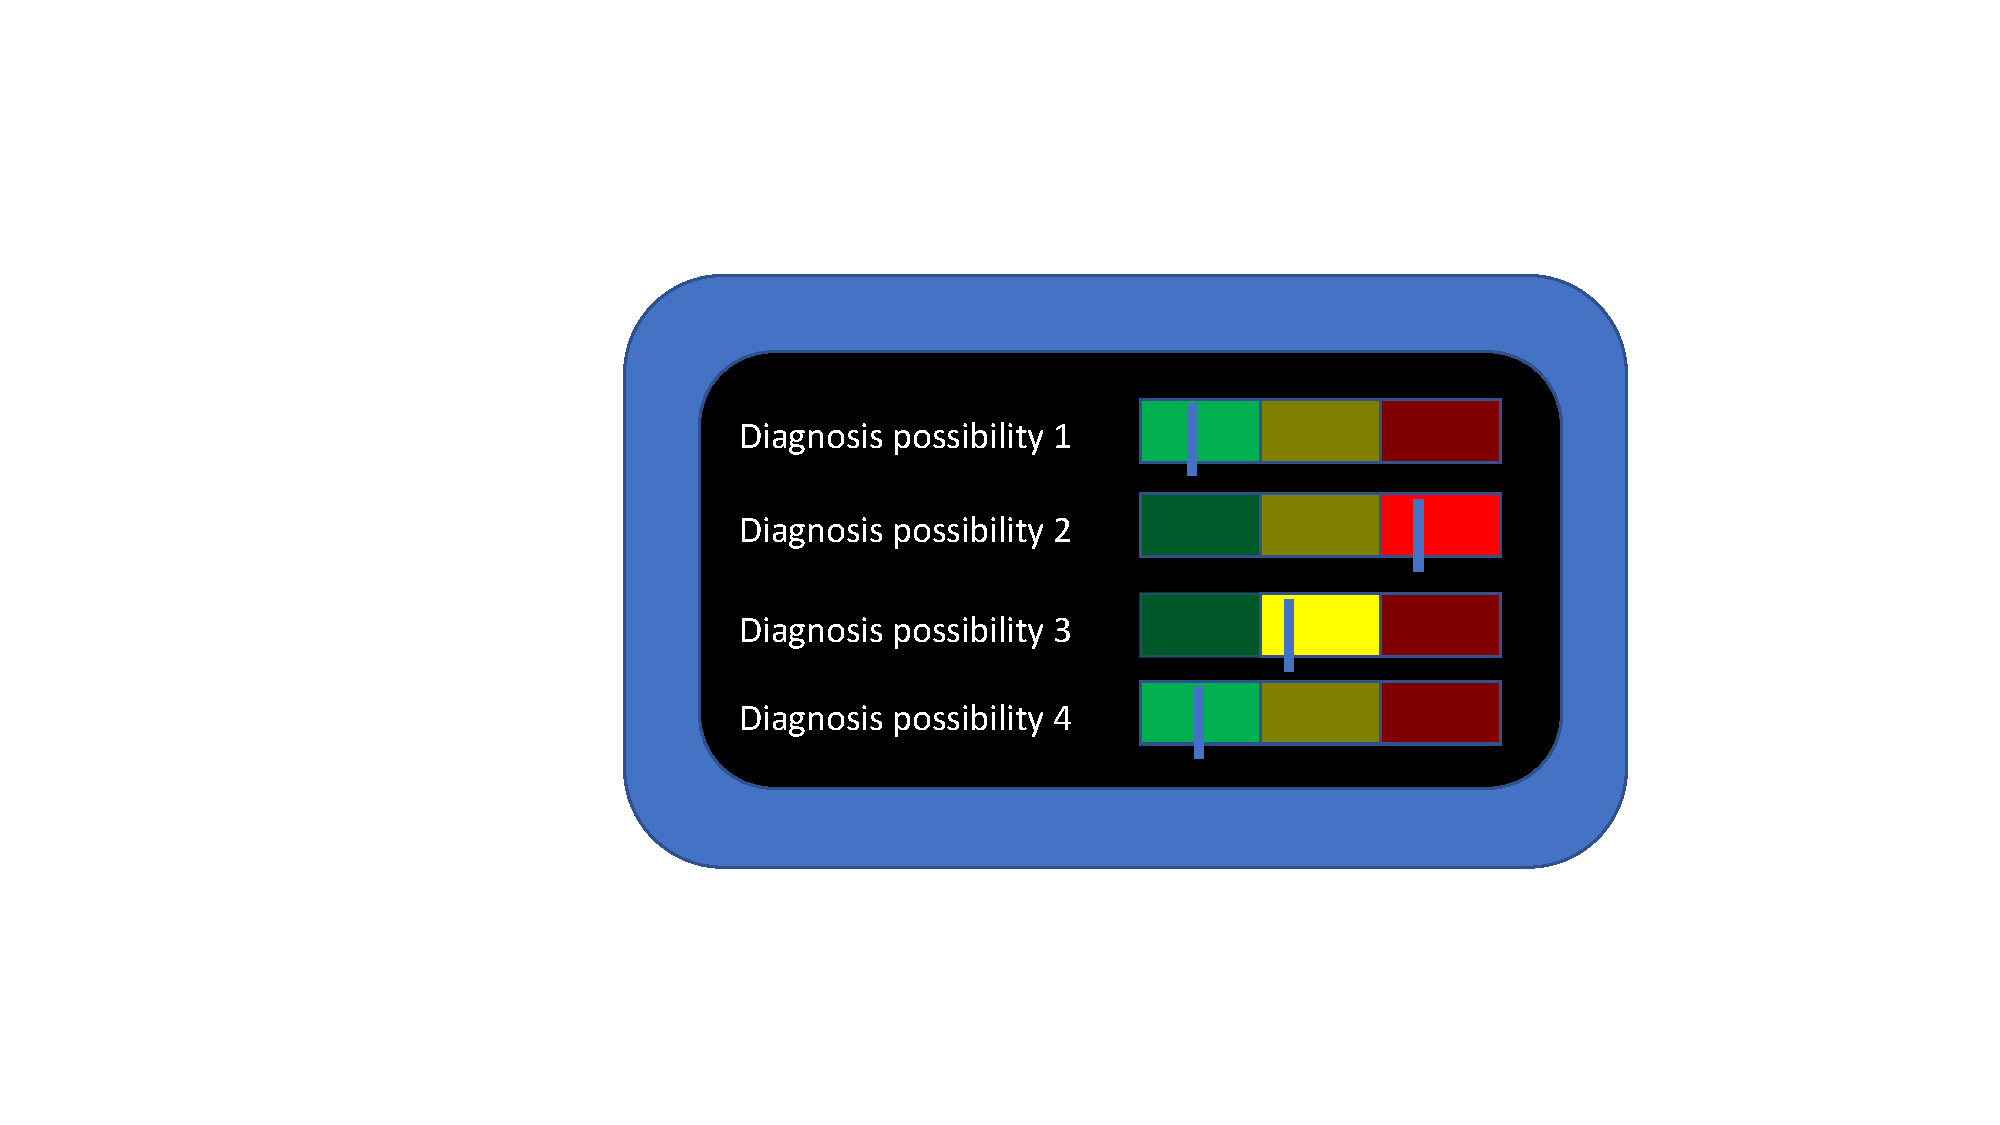
\includegraphics[width=3in]{figures/RedYellowGreen.pdf}
\end{center}
\end{figure}

  For IA technology to be widely adopted, the nurses and doctors that
  use them should experience an improvement in their practice. Suppose
  that the display of the diagnostics computer uses a three color code
  for each . Green indicates a confident
  negative diagnostic, red corresponds to a confident positive
  diagnosis. Finally, yellow corresponds to IDK, meaning that the
  computer cannot confirm or reject the diagnostic outcome.

  The thresholds which define the three ranges .... 


  
  We finish this section with a few application areas which seem ready
  for applications of IA.
  
\begin{itemize}
\item{\bf Computer aided diagnostics for large-scale data}\\
  Medical imaging devices such at digital X-ray, CT, EMR and scanning
  microscope generate many gigabytes of data for each
  patient. Radiologists and pathologists spend their days analyzing
  these images to diagnose the patient. The large size and high
  resolution of the images on the one hand, and the time limitation on
  the analyst on the other imply that the analyst has to quickly
  narrow down the suspicious region, increase the chance of missing
  dangerous abonormalities.

  IA can help the pathologist by suggesting locations in the high
  resolution image that might contain cancer nodules~\cite{}.

  directing her attention to the
  parts of the image that are 

\item{\bf Adaptive Patient montors}
  
\item {\bf Dissemination of expertise}
Computers, trained by experts, can help novices.  Serves a function
similar to score-cards.

Teaching young diagnostics
\end{itemize}

\section{Summary}

%\bibliographystyle{alpha} 
\bibliography{medbib}

\end{document}